\documentclass[10pt,onesize,a4paper,titlepage]{article}

\input{setup/preamble.sty}
\input{setup/macros.sty}

% this template consists of 3 files
% - main .tex file  (this)
% - preamble.sty    packages and color definitions
% - macros.sty      defines the macros for the entries

\begin{document}
    %%% TItle %%%
    \begin{tcolorbox}[height=0.19\textheight,colframe=accent,colback=lightgrey]
        \begin{minipage}{0.81\textwidth} % Name and Contact Info
            \vspace{4em}
            \name{Matteo Pignataro}{}
            \vspace{2em}
            \email{matteo.pignataro@tiscali.it} %$\cdot$
            \phone{Redacted} \par \vspace{0.5em}
            \address{Redacted} %$\cdot$
            \github{https://github.com/trainer400}{Matteo Pignataro}
        \end{minipage}
        \begin{minipage}{0.177\textwidth} % Picture Area
            \begin{tikzpicture}
                \begin{scope}
                    \clip [rounded corners=.5cm] (0,0) rectangle coordinate (centerpoint) (3.5,4.5cm); 
                    \node [inner sep=0pt] at (centerpoint) {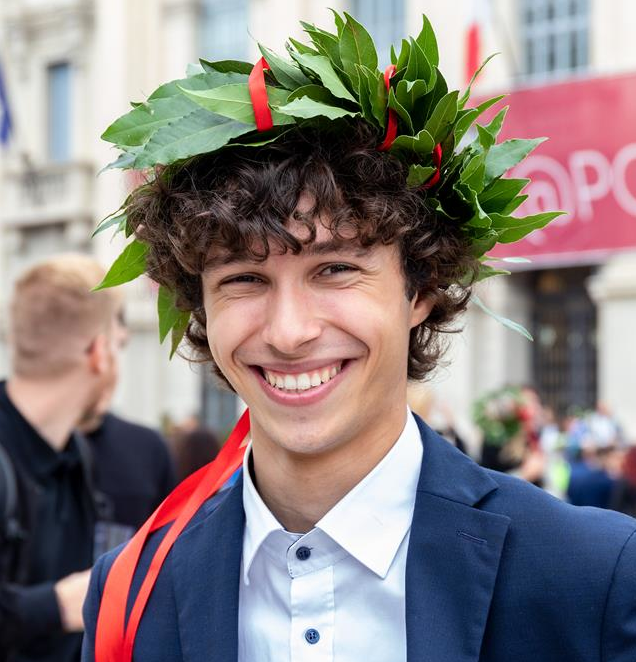
\includegraphics[width=5.0cm]{Graphics/LaureaCut.png}}; 
                \end{scope}
            \end{tikzpicture}
        \end{minipage} \hfill
    \end{tcolorbox}

    %%% Sections %%%
    \begin{tcolorbox}[grow to left by=0.55cm,colframe=white,colback=white]

        %%%%%%%%%%%% Education %%%%%%%%%%%%
        \mySection{Education}

        \entryDesc{09.2022 - 12.2025}
        {Master of Computer Science and Engineering}{at Politecnico di Milano}
        {\begin{compactitem}[-]
            \item {Final Mark: 110/110 with honors}
            \item {Thesis Title: A Scalable and Bandwidth-Aware Telemetry Framework for Autonomous Racing Vehicles}
        \end{compactitem}
        }

        \entryDesc{09.2019 - 09.2022}
        {Bachelor of Computer Science and Engineering}{at Politecnico di Milano}
        {\begin{compactitem}[-]
            \item Final Mark: 105/110
        \end{compactitem}
        }
    
        \entryDesc{09.2014 - 06.2019}
        {High School Diploma in Computer Science}{at I.T.I.S. Stanislao Cannizzaro}
        {\begin{compactitem}[-]
            \item {Final Mark: 100/100 with honors}
        \end{compactitem}}
    \end{tcolorbox}
    
    \vspace{-1cm}
    \begin{tcolorbox}[grow to left by=0.55cm,colframe=white,colback=white]
        %%%%%%%%%%%% Work experience %%%%%%%%%%%%
        \mySection{Work experience}
        \entryFocusDescWithPhoto{02.2025 - 12.2025}
        {Thesis Student}{at PoliMOVE Racing Team}
        {
            Pursued a Master’s degree in Computer Science and Engineering, with a thesis focused on flexible and bandwidth-aware smart telemetry framework for autonomous racing within the PoliMOVE research group. Experienced frequent international travel as part of the team, including extended technical trips and competitions abroad. On July 24th, the team achieved a historic milestone by securing the first place in the inaugural american road-course autonomous race at Laguna Seca Speedway in California.
        }
        {Graphics/PolimoveLogo.pdf}{1.8cm}{0.6cm}{0cm}{3.1cm 0 0 0}
    \end{tcolorbox}
    \vspace{-0.75cm}
    \begin{tcolorbox}[grow to left by=0.55cm,colframe=white,colback=white]

        \entryFocusDescWithPhoto{09.2023 - 10.2024}
        {Project Manager}{at Skyward Experimental Rocketry}
        {
            Worked as Project Manager for the Lyra rocket, coordinating a multidisciplinary team of technical leaders in designing and building a paraffin-based sounding rocket. Managed project deadlines and coordinated the work and the team to ensure the rocket was competition-ready. On September 14th, the rocket was successfully test-launched in Roccaraso, performing as expected and confirming the design's quality. Served as team leader at the European Rocketry Challenge (EuRoC) in Portugal, where the team secured the first place, winning the competition with a perfectly nominal flight.
        }
        {Graphics/SkywardLogo.png}{0.8cm}{0.35cm}{1.05cm}{-4.5cm 0 0 0}
    \end{tcolorbox}
    \vspace{-0.75cm}
    \begin{tcolorbox}[grow to left by=0.55cm,colframe=white,colback=white]

        \entryFocusDescWithPhoto{09.2022 - 09.2023}
        {Software Team Leader}{at Skyward Experimental Rocketry}
        {
            Worked as Software Team Leader for the Gemini Project. Managed a team of 15 people to program and test the first ever launched student hybrid sounding rocket in Italy. Worked closely with the electronics department to review hardware specifications and schematics. Programmed the flight software for the Main on-board computer and the whole ground refueling and ignition system. Studied, developed, and implemented a custom communication protocol between the Ground Station and the Ground Segment Equipment to guarantee collision avoidance for low-rate radio half-duplex communications.
            \newline
            \newline Achieved the following goals: 
            {
                \begin{compactitem}[-]
                    \item Learned the criticalities of managing a group of people;
                    \item Developed an interconnected system of 4 computers via CAN bus communication;
                    \item Solved complex low-level problems through the usage of oscilloscopes and logic analyzers;
                    \item Learned the dynamics of the design process as part of the technical team;
                    \item Learned the working principles of a hybrid rocket engine along with its needs in terms of software features;
                    \item Led the launch procedures for the hybrid rocket as flight controller.
                    \newline
                \end{compactitem}
            }
        }
        {Graphics/SkywardLogo.png}{0.8cm}{0.35cm}{1.05cm}{-4.5cm 0 0 0}
    \vspace{-0.75cm}
    \end{tcolorbox}
    \begin{tcolorbox}[grow to left by=0.55cm,colframe=white,colback=white]

        \entryFocusDescWithPhoto{10.2021 - 09.2022}
        {Software Team Member}{at Skyward Experimental Rocketry}
        {
            Worked as part of the software and control team for the Pyxis Project. Programmed the flight software for the Payload bay computer and worked with the Recovery team during parafoil testing for flight characterization and control algorithm tuning. Have been part of the team which traveled to Portugal to launch Pyxis at the European Rocketry Challenge (EuRoC), settling the absolute first place and winning the competition with a nominal flight.  
            \newline
            \newline Achieved the following goals:
            {
                \begin{compactitem}[-]
                    \item Worked with an embedded system developed around the STM32F429 microcontroller;
                    \item Worked with a real-time operating system (Miosix) and learning debugging with the gdb tool;
                    \item Familiarized with standard communication protocols: SPI, UART, I2C, and CAN;
                    \item Learned how to write device drivers from data sheets and user manuals;
                    \item Learned the basics of a Hardware-In-the-Loop (HIL) simulation;
                    \item Learned the fundamentals of a sounding rocket flight and team working;
                    \item Became familiar with the significant importance of procedures and checklists.
                \end{compactitem}
            }
        }
        {Graphics/SkywardLogo.png}{0.8cm}{0.35cm}{1.05cm}{-4.5cm 0 0 0}
    \end{tcolorbox}

    \centering{
        % The % symbols are mandatory
        \begin{minipage}{0.30 \linewidth}
            \begin{tcolorbox}[height=0.22\textheight, width=0.8\textwidth, grow to right by=0.5cm, colback=accent!60!white,colframe=accent,arc=1mm]
                \vspace{0.5em}
                \subsection*{Programming Skills}
                    \skill{C}{5}
                    \skill{C++}{4}
                    \skill{Java}{4}
                    \skill{Python}{4}
            \end{tcolorbox}
        \end{minipage}%
        %
        \begin{minipage}{0.30 \linewidth}
            \begin{tcolorbox}[height=0.22\textheight, width=0.8\textwidth,grow to right by=0.5cm, colback=accent!60!white,colframe=accent,arc=1mm]
                \vspace{0.5em}
                \subsection*{Language Skills}
                    \skill{Italian}{5}
                    \skill{English (Writing)}{3}
                    \skill{English (Speaking)}{4}
            \end{tcolorbox}
        \end{minipage}%
        %
        \begin{minipage}{0.30 \linewidth}
            \begin{tcolorbox}[height=0.22\textheight, width=0.8\textwidth,grow to right by=0.5cm, colback=accent!60!white,colframe=accent,arc=1mm]
                \vspace{0.5em}
                \subsection*{Other Skills}
                    \skill{CAD (CREO Parametric)}{3}
                    \skill{Electronics}{4}
                    \skill{Hand Soldering}{4}
                    \skill{LaTeX}{3}
            \end{tcolorbox}
        \end{minipage}%
        }

    \begin{tcolorbox}[grow to left by=0.55cm,colframe=white,colback=white]
        %%%%%%%%%%%% Certificates %%%%%%%%%%%%
        \mySection{Certificates}
        \entry{04.2022}{Test of English for International Communication (TOEIC): B2 (955 points)}
        \entry{05.2018}{Cambridge First Certificate (FCE): B1}
        \entry{06.2017}{Cambridge Preliminary Certificate (PET): B1}
    \end{tcolorbox}

    \vspace{-1cm}
    \begin{tcolorbox}[grow to left by=0.55cm,colframe=white,colback=white]
        %%%%%%%%%%%% Interests %%%%%%%%%%%%
        \mySection{Interests}
        \entryFocusDescWithPhoto{}
        {Computer Graphics}{}
        {
            One of main interests is computer graphics. Studied and used the Vulkan and OpenGL APIs and to write a low-level, object-oriented framework for them. Also designed a 3D visualizer for rocket trajectory and attitude to better visualize flights from the ground station.
        }
        {Graphics/VulkanLogo.png}{1.25cm}{0.0cm}{0cm}{0 0 0 0}
    \end{tcolorbox}
    
    \vspace{-0.75cm}
    \begin{tcolorbox}[grow to left by=0.55cm,colframe=white,colback=white]
        %%%%%%%%%%%% Interests %%%%%%%%%%%%
        \entryFocusDescWithPhoto{}
        {Electronics}{}
        {
            Passionate of analog and digital electronics. At university studied the fundamentals of electronics and completed a course in digital electronics design. Additionally, completed Radio amateur certification and have experience with hand soldering down to 0201 form factor components. Presented twice at the Rome Maker Faire showcasing two high-voltage projects. Through these experiences, learned the usage of essential electronics instrumentation such as oscilloscopes, logic analyzers, and function generators, which enabled me to design and build analog amplifiers and multiple solid-state Tesla coils at home.
            Currently part of IoT project to develop Matter mesh-connected wall sockets and working with embedded real time OS.
        }
        {Graphics/electronics.png}{1.25cm}{0.45cm}{0.1cm}{0 0 0 0}
    \end{tcolorbox}
\end{document}